\documentclass[a4j, 9pt]{ltjsarticle}

\usepackage{multicol}
\usepackage{amsmath}
\usepackage{tikz}
\usetikzlibrary{calc}

%label属性のついたものの背景色を白で四角系で塗りつぶす
\tikzset{set label/.style={fill=white,rectangle,inner sep=1}}

%定義記号
\def\ldef{\coloneqq}
\def\define{\stackrel{\mathrm{def}}{=}}
\def\defineProposition{\stackrel{\mathrm{def}}{\Longleftrightarrow}}

%ディスプレイスタイル
\def\ds{\displaystyle}

\setlength{\columnsep}{5mm}
\columnseprule=0.2mm

\begin{document}

\section*{\S 1写像}
  
  数学的にモデルを扱うとき集合論的に思考すると上手にそのモデルを扱うことができる。これは数学の問題を解く場合も同様である。ここでは集合間を関係づける概念、写像についてみておこう。

\begin{multicols*}{2}

  \subsubsection{写像の定義}
    $\ds X, Y$を空でない集合とする。\par
    任意の$\ds x \in X$に対し、ある$\ds y \in Y$が一意に定まるとき、このような対応規則を「$\ds X$から$\ds Y$への写像」と呼ぶ。\par
    また$\ds X, Y$が数を要素とする集合の場合特に関数と呼ぶ。つまり$\ds 関数 \subset 写像$である。\par
    簡潔に表現すれば以下。

    \vspace{9pt}\\

    $\ds f:X \mapsto Y \defineProposition \forall_{x \in X} [\exists!_{y \in Y} [y = f(x)]]$

    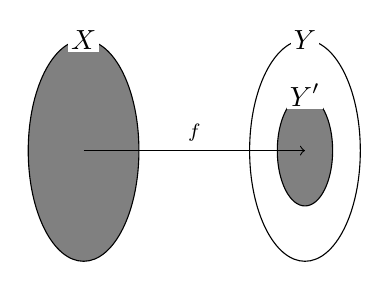
\begin{tikzpicture}[auto]
      
      %Xのベン図
      \fill[color=black!50!white, draw=black] (0,0) ellipse (20pt and 40pt);
      \node[set label,text=black] (X) at (0, 40pt) {$\ds X$};

      %Yのベン図
      \draw (80pt,0) ellipse (20pt and 40pt);
      \fill[color=black!50!white, draw=black] (80pt, 0) ellipse (10pt and 20pt); % black!50!white で黒と白50%
      \node[set label,text=black] (Y) at (80pt, 40pt) {$\ds Y$};
      \node[set label,text=black] (Y') at (80pt, 20pt) {$\ds Y'$};

      %写像f
      \draw[->] (0, 0) to node {$\scriptstyle f$} (80pt, 0);

    \end{tikzpicture}

  \subsubsection{定義域・値域}
    $\ds f:X \mapsto Y$において\par
    \begin{cases}
      $\ds X$を$\ds f$の定義域\\
      $\ds Y'(\subset Y)$を$\ds f$の値域\\
    \end{cases}
    という。\par

    値域$\ds R_f$の具体的な定義は以下。
    
    \vspace{9pt}\\

    $\ds R_f \defineProposition \{y \in Y \mid \exists_x [x \in X \wedge y=f(x)]\}$

    % \footnote{
    %   $\ds \exists_x [x \in X \wedge y=f(x)]$は自由変項$\ds y$が残るため$\ds y$の条件と言える。
    % }

  \subsubsection{単射(行先がかぶらない写像)}
    写像にはいくつか特性が存在する。その特性の一つを有する写像が単射と呼ばれるものである。\par
    $\ds f:X \mapsto Y$が単射であるとは、任意の$x,x'\in X$に対して「$\ds x \ne x' \Longrightarrow f(x) \ne f(x')$」が成立することである。\par
    つまり簡潔に表せば以下。

    \begin{equation}
      \begin{split}\notag
          $\ds f:X \mapsto Yが単射$     & $\defineProposition      \forall_{x,x'\in X} [x \ne x' \Longrightarrow f(x) \ne f(x')]$\\
                                        & $\ds \Longleftrightarrow  \forall_{x,x'\in X} [f(x) = f(x') \Longrightarrow x = x']$\\
      \end{split}
    \end{equation}

    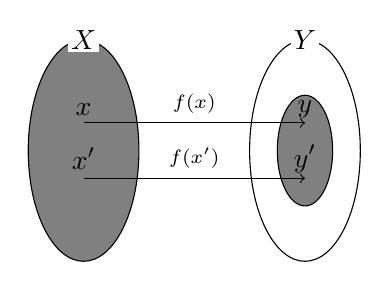
\begin{tikzpicture}[auto]
      
      %Xのベン図
      \fill[color=black!50!white, draw=black] (0,0) ellipse (20pt and 40pt);
      \node[set label, text=black] (X) at (0, 40pt) {$\ds X$};

      %Yのベン図
      \draw (80pt,0) ellipse (20pt and 40pt);
      \fill[color=black!50!white, draw=black] (80pt, 0) ellipse (10pt and 20pt); % black!50!white で黒と白50%
      \node[set label, text=black] (Y) at (80pt, 40pt) {$\ds Y$};

      %x->y
      \node (x) at (0, 15pt) {$\ds x$};
      \node (y) at (80pt, 15pt) {$\ds y$};
      \draw[->] (0, 10pt) to node {$\scriptstyle f(x)$} (80pt, 10pt);

      %x'->y'
      \node (x') at (0, -3pt) {$\ds x'$};
      \node (y') at (80pt, -3pt) {$\ds y'$};
      \draw[->] (0, -10pt) to node {$\scriptstyle f(x')$} (80pt, -10pt);

    \end{tikzpicture}

  \subsubsection{全射}
    写像の特使の一つを有するものを単射と言った。他にも全射と呼ばれるものもある。\par
    $\ds f:X \mapsto Y$が全射であるとは、任意の$y \in Y$に対して、ある$\ds x \in X$が存在し$\ds f(x)=y$となることである。\par
    つまり簡潔に表せば以下。

    \begin{equation}
      \begin{split}\notag
          $\ds f:X \mapsto Yが全射$     & $\defineProposition      \forall_{y\in Y} [\exists_{x\in X} [f(x) = y]]$\\
      \end{split}
    \end{equation}

    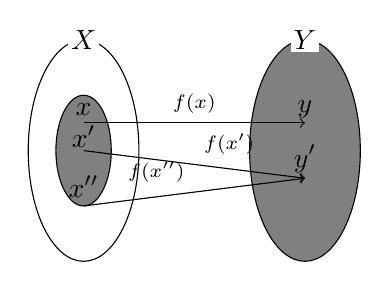
\begin{tikzpicture}[auto]
      
      %Xのベン図
      \draw (0,0) ellipse (20pt and 40pt);
      \fill[color=black!50!white, draw=black] (0, 0) ellipse (10pt and 20pt); % black!50!white で黒と白50%
      \node[set label, text=black] (X) at (0, 40pt) {$\ds X$};

      %Yのベン図
      \fill[color=black!50!white, draw=black] (80pt,0) ellipse (20pt and 40pt);
      \node[set label, text=black] (Y) at (80pt, 40pt) {$\ds Y$};

      %x->y
      \node (x) at (0, 15pt) {$\ds x$};
      \node (y) at (80pt, 15pt) {$\ds y$};

      %x'->y'
      \node (x') at (0, 5pt) {$\ds x'$};
      \node (y') at (80pt, -3pt) {$\ds y'$};

      %x''->y'
      \node (x'') at (0, -13pt) {$\ds x''$};

      \draw[->] (0, 10pt) to node {$\scriptstyle f(x)$} (80pt, 10pt);
      \draw[->] (0, 0) to node {$\scriptstyle f(x')$} (80pt, -10pt);
      \draw[->] (0, -20pt) to node {$\scriptstyle f(x'')$} (80pt, -10pt);

    \end{tikzpicture}

    \subsubsection{全単射(1対1対応、変換)}
    既に写像の特性を持つものを2つ紹介したが、これらの特性を同時に有する者ももちろん存在する。それを全単射といい、単射と全射それぞれの定義から成る合成命題で定義される。\par
    $\ds f:X \mapsto Y$が全単射であるとは、$\ds f$が単射かつ全射であるときをいう。\par
    また、定義域と値域が等しいことよりこの対応を1対1対応とも呼び、さらに互いの集合間をすべての要素が行き来できることより変換とも呼ぶ。\par
    つまり簡潔に表せば以下。

    \begin{multline*}
        $\ds f:X \mapsto Yが全単射 \defineProposition \forall_{x,x'\in X} [f(x) = f(x') \Longrightarrow x = x']$\\
                                                      $\ds \wedge \forall_{y\in Y} [\exists_{x\in X} [f(x) = y]]$
    \end{multline*}

    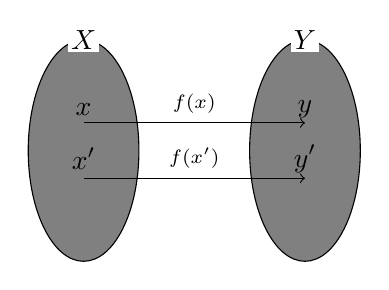
\begin{tikzpicture}[auto]
      
      %Xのベン図
      \fill[color=black!50!white, draw=black] (0,0) ellipse (20pt and 40pt);
      \node[set label, text=black] (X) at (0, 40pt) {$\ds X$};

      %Yのベン図
      \fill[color=black!50!white, draw=black] (80pt,0) ellipse (20pt and 40pt);
      \node[set label, text=black] (Y) at (80pt, 40pt) {$\ds Y$};

      %x->y
      \node (x) at (0, 15pt) {$\ds x$};
      \node (y) at (80pt, 15pt) {$\ds y$};
      \draw[->] (0, 10pt) to node {$\scriptstyle f(x)$} (80pt, 10pt);

      %x'->y'
      \node (x') at (0, -3pt) {$\ds x'$};
      \node (y') at (80pt, -3pt) {$\ds y'$};
      \draw[->] (0, -10pt) to node {$\scriptstyle f(x')$} (80pt, -10pt);

    \end{tikzpicture}

\end{multicols*}

\end{document}
